\documentclass[12pt]{article}
\usepackage[T1, T2A]{fontenc}
\usepackage[utf8]{inputenc}
\usepackage[russian]{babel}
\usepackage{hyperref}
\usepackage{graphicx}
\graphicspath{ {../Images/} }

\author{Григорий Матюхин}
\date{\today}
\title{Лабораторная работа \textnumero14.\\Партиции, файловые системы, монтирование}

\begin{document}
\maketitle
\newpage
\tableofcontents
\newpage
\section{Цель работы}
Получить навыки создания разделов на диске и файловых систем. Получить навыки монтирования файловых систем.

\section{Последовательность выполнения работы}
\subsection{Создание разделов MBR с помощью \texttt{fdisk}}
\begin{enumerate}
	\item Запустите вашу виртуальную машину с добавленными дополнительными дисками
	\item В командной строке с полномочиями администратора с помощью \texttt{fdisk} посмотрите перечень разделов на всех имеющихся в системе устройствах жёстких дисков:
	      \\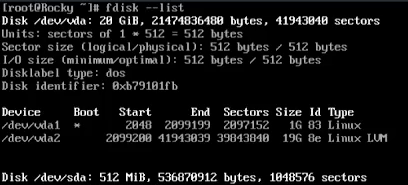
\includegraphics{1.png}
	\item Предположим, что необходимо сделать разметку диска \texttt{/dev/sdb} с помощью утилиты \texttt{fdisk}:
	\item Введите \texttt{m}, чтобы получить справку по командам:
	\item Нажмите \texttt{p}, чтобы просмотреть текущее распределение пространства диска:
	\item Введите \texttt{n}, чтобы добавить новый раздел;
	\item Выберите \texttt{p}, чтобы создать основной раздел:
	\item Укажите первый сектор на диске, с которого начнётся новый раздел:
	\item Укажите последний сектор, которым будет завершён раздел. Например, введите \texttt{+100M}, чтобы создать раздел на 100 MiB:
	\item На этом этапе можно определить тип раздела. Нажмите \texttt{Enter}, чтобы принять тип раздела по умолчанию 83:
	\item Нажмите \texttt{w}, чтобы записать изменения на диск и выйти из \texttt{fdisk}:
	      \\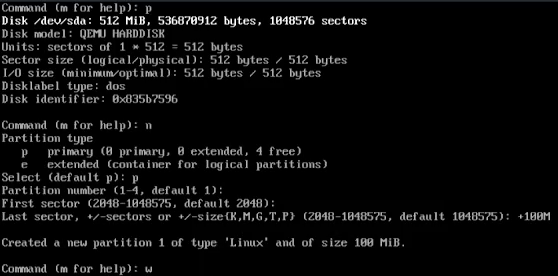
\includegraphics{2.png}
	\item Запишите изменения в таблицу разделов ядра:
\end{enumerate}

\subsection{Создание логических разделов}
\begin{enumerate}
	\item В терминале с полномочиями администратора запустите \texttt{fdisk}:
	\item Введите \texttt{n}, чтобы добавить новый раздел:
	\item Введите \texttt{e}, чтобы создать расширенный раздел:
	\item Нажмите \texttt{Enter}, чтобы принять первый сектор по умолчанию и снова нажмите \texttt{Enter}, когда \texttt{fdisk} запросит последний сектор:
	\item Из интерфейса \texttt{fdisk} снова нажмите \texttt{n}:
	\item Нажмите \texttt{Enter}, чтобы принять выбор первого сектора в качестве сектора по умолчанию. На вопрос о последнем секторе введите \texttt{+101M}:
	\item После создания логического раздела введите \texttt{w}, чтобы записать изменения на диск и выйти из \texttt{fdisk}.
	      \\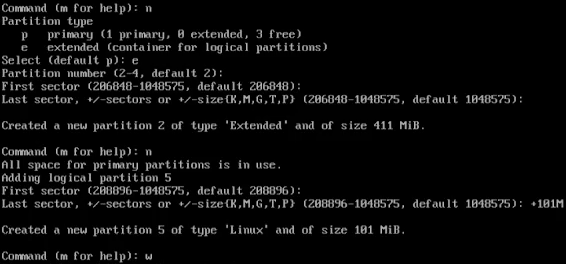
\includegraphics{3.png}
\end{enumerate}

\subsection{Создание раздела подкачки}
\begin{enumerate}
	\item Получите полномочия администратора. Запустите \texttt{fdisk}:
	\item Нажмите \texttt{n}, чтобы добавить новый раздел.
	\item Нажмите \texttt{Enter}, чтобы принять первый сектор по умолчанию. На вопрос о последнем секторе введите \texttt{+100M}.
	\item Далее измените тип раздела. Для этого нажмите \texttt{t}, затем укажите номер партиции, для которой хотите изменить тип.
	      Затем введите код типа раздела (в данном случае 82 — раздел подкачки).
	\item После создания логического раздела введите \texttt{w}, чтобы записать изменения на диск и выйти из \texttt{fdisk}.
	      \\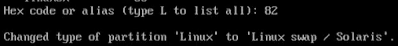
\includegraphics{4.png}
	\item Просмотрите информацию о добавленных разделах:
	\item Отформатируйте раздел подкачки:
	\item Для включения вновь выделенного пространства подкачки используйте:
	\item Для просмотра размера пространства подкачки, которое в настоящее время выделено, введите \texttt{free -m}.
	      \\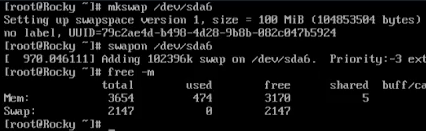
\includegraphics{5.png}
\end{enumerate}

\subsection{Создание разделов GPT с помощью \texttt{gdisk}}
\begin{enumerate}
	\item В терминале с полномочиями администратора с помощью \texttt{gdisk} посмотрите таблицы разделов и разделы на втором добавленном вами ранее диске \texttt{/dev/sdb}:
	\item Создайте раздел с помощью \texttt{gdisk}:
	\item Введите \texttt{n}, чтобы добавить новый раздел:
	\item Теперь вас попросят задать первый сектор. Чтобы создать раздел диска размером 100 MiB, используйте \texttt{+100M}:
	\item Теперь предлагается установить тип раздела. Можно просто нажать \texttt{Enter}, чтобы принять тип раздела 8300 (Linux) по умолчанию:
	      \\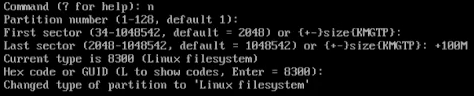
\includegraphics{6.png}
	\item Теперь раздел создан. Нажмите \texttt{p}, чтобы отобразить разбиение диска:
	\item Если текущее разбиение устраивает, нажмите \texttt{w}, чтобы записать изменения на диск:
	\item Обновите таблицу разделов:
	\item Просмотрите информацию о добавленных разделах:
\end{enumerate}

\subsection{Форматирование файловой системы XFS}
\begin{enumerate}
	\item В терминале с полномочиями администратора для диска \texttt{/dev/sda1} создайте файловую систему XFS:
	\item Для установки метки файловой системы в \texttt{xfsdisk} введите
	      \\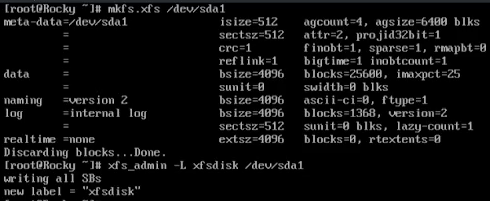
\includegraphics{7.png}
\end{enumerate}

\subsection{Форматирование файловой системы EXT4}
\begin{enumerate}
	\item В терминале с полномочиями администратора для диска \texttt{/dev/sda5} создайте файловую систему EXT4:
	\item Для установки метки файловой системы в \texttt{ext4disk} введите
	\item Для установки параметров монтирования по умолчанию для файловой системы введите
	      \\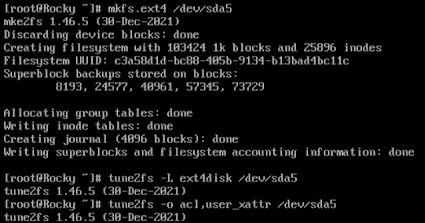
\includegraphics{8.png}
\end{enumerate}

\subsection{Ручное монтирование файловых систем}
\begin{enumerate}
	\item Получите полномочия администратора. Для создания точки монтирования для раздела введите:
	\item Чтобы смонтировать файловую систему, используйте следующую команду:
	      \\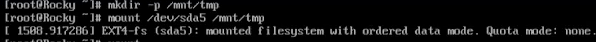
\includegraphics{9.png}
	\item Чтобы отмонтировать раздел, можно использовать umount либо с именем устройства, либо с именем точки монтирования:
	      \\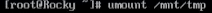
\includegraphics{10.png}
\end{enumerate}

\subsection{Монтирование разделов с помощью \texttt{/etc/fstab}}
\begin{enumerate}
	\item Получите полномочия администратора:
	\item Создайте точку монтирования для раздела XFS \texttt{/dev/sda1}:
	\item Посмотрите информацию об идентификаторах блочных устройств (UUID):
	\item Введите \texttt{blkid /dev/sda1} и скопируйте значение идентификатора UUID для устройства \texttt{/dev/sda1}:
	\item Откройте файл \texttt{/etc/fstab} на редактирование и добавьте следующую строку:
	      \texttt{UUID=<partition-uuid> /mnt/data xfs defaults 1 2}
	      \\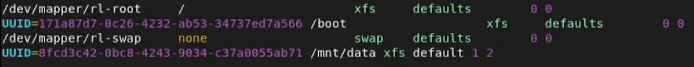
\includegraphics{11.png}
	\item Перед попыткой автоматического монтирования при перезагрузке рекомендуется проверить конфигурацию.
	      Следующая команда монтирует всё, что указано в \texttt{/etc/fstab}:
	\item Проверьте, что раздел примонтирован правильно:
	      \\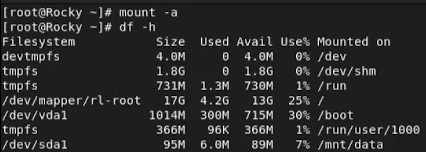
\includegraphics{12.png}
\end{enumerate}

\subsection{Самостоятельная работа}
\begin{enumerate}
	\item Добавьте две партиции на диск с разбиением GPT.
	      Создайте оба раздела размером 100 MiB.
	      Один из этих разделов должен быть настроен как пространство подкачки, другой раздел должен быть отформатирован файловой системой ext4.
	      \\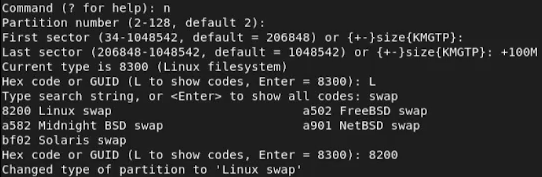
\includegraphics{13.png}
	      \\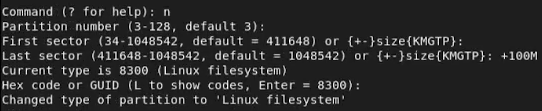
\includegraphics{14.png}
	\item Настройте сервер для автоматического монтирования этих разделов.
	      Установите раздел ext4 на \texttt{/mnt/data-ext} и установите пространство подкачки в качестве области подкачки.
	      \\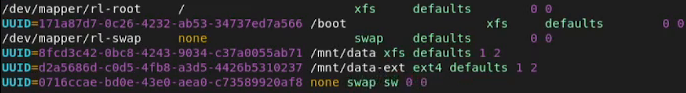
\includegraphics{15.png}
	\item Перезагрузите вашу систему и убедитесь, что всё установлено правильно.
	      \\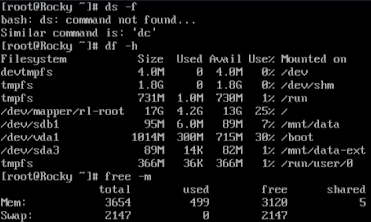
\includegraphics{16.png}
\end{enumerate}

\section{Контрольные вопросы}
\begin{enumerate}
	\item Какой инструмент используется для создания разделов GUID? \\
	      \texttt{gdisk}
	\item Какой инструмент применяется для создания разделов MBR? \\
	      \texttt{fdisk}
	\item Какая файловая система используется по умолчанию для систем типа RHEL? \\
	      XFS
	\item Какой файл используется для автоматического монтирования разделов во время загрузки? \\
	      \texttt{/etc/fstab}
	\item Какой вариант монтирования целесообразно выбрать, если необходимо, чтобы файловая система не была автоматически примонтирована во время загрузки? \\
	      Монтировать вручную.
	\item Какая команда позволяет форматировать раздел с типом 82 с соответствующей файловой системой? \\
	      \texttt{mkswap <partition>}
	\item Вы только что добавили несколько разделов для автоматического монтирования при загрузке.
	      Как можно безопасно проверить, будет ли это работать без реальной перезагрузки? \\
	      Используя \texttt{mount -a} примонтировать все содержимое \texttt{/etc/fstab} и проверить правильность с помощью \texttt{df -h}.
	\item Какая файловая система создаётся, если вы используете команду \texttt{mkfs} без какой-либо спецификации файловой системы? \\
	      Ext2
	\item Как форматировать раздел EXT4? \\
	      \texttt{mkfs.ext4 <partition>}
	\item Как найти UUID для всех устройств на компьютере? \\
	      \texttt{blkid}
\end{enumerate}

\section{Вывод}
В ходе выполнения данной работы я получил навыки создания разделов на диске и файловых систем и навыки монтирования файловых систем.

\end{document}
